\documentclass[11pt,a4paper]{amsart}
\usepackage[utf8]{inputenc}
\usepackage[T1]{fontenc}
\usepackage{amsmath,amssymb,amsthm}
\usepackage{booktabs}
\usepackage{graphicx}
\usepackage{array}
\usepackage{enumitem}
\usepackage[margin=1in]{geometry}
\usepackage{xcolor}
\usepackage{hyperref}
\hypersetup{colorlinks=true,linkcolor=blue!60!black,citecolor=blue!60!black,urlcolor=blue!60!black}

\newtheorem{theorem}{Theorem}[section]
\newtheorem{proposition}[theorem]{Proposition}
\newtheorem{lemma}[theorem]{Lemma}
\newtheorem{corollary}[theorem]{Corollary}
\newtheorem{conjecture}[theorem]{Conjecture}
\theoremstyle{definition}
\newtheorem{definition}[theorem]{Definition}
\newtheorem{remark}[theorem]{Remark}
\newtheorem{example}[theorem]{Example}

\newcommand{\F}{\mathbb{F}}
\newcommand{\Z}{\mathbb{Z}}
\newcommand{\A}{\mathbb{A}}
\newcommand{\G}{\mathcal{G}}
\newcommand{\Tr}{\operatorname{Tr}}
\newcommand{\Var}{\operatorname{Var}}
\newcommand{\Arf}{\operatorname{Arf}}
\newcommand{\im}{\operatorname{im}}
\newcommand{\Frob}{\operatorname{Frob}}
\newcommand{\charpoly}{\operatorname{charpoly}}
\newcommand{\eps}{\varepsilon}
\newcommand{\sgn}{\varepsilon_0}

\title[Legendre intervals in even characteristic, II]{Prime polynomials in Legendre intervals over $\F_{2^k}[t]$, II:\\ exact variances via quadratic towers and supersingular Artin--Schreier curves}

\author{Ruqing Chen}
\address{GUT Geoservice Inc., Montreal, Canada}
\email{ruqing@hotmail.com}
\thanks{Preprint. Zenodo DOI: \href{https://doi.org/10.5281/zenodo.23224897}{10.5281/zenodo.23224897}. Code and data: \url{https://github.com/Ruqing1963/legendre-intervals-part2}.}
\date{\today}

\begin{document}

\begin{abstract}
Let $q=2^k$ and let $\mathcal I_f=\{f^2+s:\deg s\le d\}$ be the Legendre interval of a monic $f\in\F_q[t]$ of degree $d$. Chen's Open Problem~8.2 asks why the variance of the prime-power count $\Psi(f)=\sum_{P\in\mathcal I_f}\Lambda(P)$ deviates by a factor as large as $q^2/3$ from the Keating--Rudnick prediction. We resolve the case $d=4$ completely and unconditionally: using the quadratic tower $\F_q\subset\F_{q^2}\subset\F_{q^4}\subset\F_{q^8}$ we obtain a closed formula for $\Psi$ on every class of the Hayes group $\G_3$, from which $\Var_{\G^2}(\Psi)/q^5=q(q-1)$, $\Var_{\G}(\Psi)/q^5=3-3/q$, the full structure of the quadratic-twist correlations, and an elementary proof of Carlitz's cubic evaluation over $\F_{2^{8k}}$ follow. For $d=6$ we prove that the Legendre profile takes exactly three values governed by $[c_2=0]$ and $\Tr(c_4/c_2^2)$, reducing the variance to three exponential sums $A_6,X,Y$ on $U=\{\alpha\in\F_{q^{12}}:\Tr\alpha=\Tr\alpha^3=\Tr\alpha^5=0\}$. We show that $A_6-q^9$ and $X$ are sums of Frobenius traces of supersingular Artin--Schreier curves $y^2+y=\lambda_5x^5+\lambda_3x^3+\lambda_1x$ and reduce them to $\F_2$-quadratic forms whose radicals are kernels of explicit linearised polynomials; their conjectured closed forms $A_6=q^9+(-1)^{k+1}(q-1)q^5$, $X=(-1)^{k+1}q^6+q^5$ are verified exactly for $q\le128$ by an algorithm independent of the explicit formula, and the pure cubic part is proved for all $k$. The third constant $Y=q^3m_k$ is a twisted Frobenius trace on a fixed nine-dimensional complete intersection $X=V(e_1,e_3,e_5)\subset\A^{12}_{\F_2}$ (geometrically integral, normal, with explicit two-dimensional singular locus) and is not a character sum; we discuss its weight and rank. Consequently the Legendre variance at $d=6$ obeys $\Var_{\G^2}/q^{7}\asymp q^2$, not $q^4$.
\end{abstract}

\maketitle
\tableofcontents

\section{Introduction}

Let $q=2^k$, $d\ge2$, $n=2d$ and $\ell=d-1$. For a monic $f\in\F_q[t]$ of degree $d$ the \emph{Legendre interval} is
\[
\mathcal I_f=\{f^2+s:\ s\in\F_q[t],\ \deg s\le d\},\qquad |\mathcal I_f|=q^{d+1},
\]
and $\Psi(f)=\sum_{P\in\mathcal I_f}\Lambda(P)$ counts prime powers in it with the von Mangoldt weight. In odd characteristic the sets $\mathcal I_f$ are ordinary short intervals and the variance of $\Psi$ is governed by the Keating--Rudnick theorem \cite{KR}, which predicts $\Var(\Psi)\sim(d-2)q^{d+1}$ as $q\to\infty$. In characteristic $2$ the squaring map on the Hayes group is a homomorphism, the Legendre intervals are the fibres over the subgroup of squares, and Chen \cite{Chen} observed (Table~4 of \emph{op.\ cit.}) that the variance over Legendre intervals exceeds the full-group variance by factors $4/3,\ 16/3,\ 64/3$ for $q=2,4,8$ at $d=4$ and asked for an explanation (Open Problem~8.2).

This paper is the second part of our study. Part~I established the dictionary between Legendre intervals and quadratic characters of the Hayes group and verified, by exact computation for $q\le8$, the identities $\Var_{\G^2}(\Psi)/q^5=q(q-1)$ and $\Var_{\G}(\Psi)/q^5=3-3/q$. Here we prove them for all $q=2^k$, and we carry the analysis to $d=6$, where a genuinely new phenomenon appears: two of the three constants that control the Legendre variance are elementary while the third is a Frobenius trace that is not a character sum.

\subsection*{Main results}
All variances below are second moments about the global mean $q^{d+1}$ (this is the quantity tabulated in \cite{Chen}); see Section~\ref{sec:prelim}.

\begin{itemize}[leftmargin=2em]
\item \textbf{$d=4$ (Section~\ref{sec:d4}).} Theorem~\ref{thm:d4formula} gives $\Psi$ on every class of the Hayes group $\G_3$ in closed form. Consequently (Theorems~\ref{thm:varH4}, \ref{thm:varG4}, \ref{thm:rho4}) for every $q=2^k$
\[
\frac{\Var_{\G^2}(\Psi)}{q^5}=q(q-1),\qquad \frac{\Var_{\G}(\Psi)}{q^5}=3-\frac3q,\qquad \frac{\Var_{\G^2}}{\Var_{\G}}=\frac{q^2}{3},
\]
the deviation $\Psi-q^5$ is supported on the subgroup $\{c_1=0\}$, the identity class carries the deficit $-(q^4-q^3)$, and the quadratic-twist correlations $\rho(\eps)$ equal $1$ on the $q-1$ characters of conductor $u^2$ and $(q-3)/(3(q-1))$ on all others when $k$ is odd.
\item \textbf{$d=6$, structure (Section~\ref{sec:d6}).} Theorem~\ref{thm:threevalue}: on the $q^2$ Legendre classes $(0,c_2,0,c_4,0)$ the function $\Psi$ takes exactly three values,
\[
\Psi(0,c_2,0,c_4,0)=q^7+\frac{A_6-q^9-X}{q^2}+\frac Xq[c_2=0]+\frac Yq[c_2\ne0]\,\chi\Big(\frac{c_4}{c_2^2}\Big),
\]
where $A_6=|U|$, $X=\sum_U\chi(e_2)$, $Y=\sum_U\chi(e_4)$ and $U=\{\alpha\in\F_{q^{12}}:\Tr\alpha=\Tr\alpha^3=\Tr\alpha^5=0\}$. The proof uses only the $\F_q$-translation and scaling symmetries of $U$.
\item \textbf{$d=6$, the constants (Sections~\ref{sec:tower6}--\ref{sec:qf}).} Theorem~\ref{thm:towerred} reduces $A_6,X,Y$ to explicit finite sums over $\F_{q^6}$. Theorem~\ref{thm:supersing} expresses $A_6-q^9$ and $X$ through the Frobenius traces of the supersingular curves $y^2+y=\lambda_5x^5+\lambda_3x^3+\lambda_1x$, equivalently through $\F_2$-quadratic forms on $\F_{q^{12}}$ with explicit radicals. Lemma~\ref{lem:purecubic} evaluates the pure cubic part for all $k$. Conjecture~\ref{conj:A6X}, verified exactly for $q\le128$ (Table~\ref{tab:A6X}), states $A_6=q^9+(-1)^{k+1}(q-1)q^5$ and $X=(-1)^{k+1}q^6+q^5$.
\item \textbf{Scaling law and $Y$ (Section~\ref{sec:Y}).} Theorem~\ref{thm:varH6} gives $\Var_{\G^2}(\Psi)/q^7$ at $d=6$ in closed form in terms of $(q,k,m_k)$, $m_k=Y/q^3$; it implies $\Var_{\G^2}/q^7\asymp q^2$ (Table~\ref{tab:d6var}) and $\lim\Var_{\G^2}/q^9=1$ provided $m_k=o(q^{5/2})$. We identify $Y$ as the trace of a twisted Frobenius $\sigma F^k$ on the cohomology of a fixed nine-dimensional complete intersection $X\subset\A^{12}_{\F_2}$ with an Artin--Schreier sheaf (Propositions~\ref{prop:trace}--\ref{prop:Xgeom}, Theorem~\ref{thm:twisted}) and show that the data $m_k=13,-1,-35,47,733$ ($k\le5$) exclude a pure weight-$3$ object of rank $\le5$.
\end{itemize}

\subsection*{Methods}
Two ideas carry the paper. The first is the \emph{quadratic tower}: for $n=2d$ the extension $\F_{q^n}/\F_{q^{n/2}}$ is quadratic, so every $\alpha\in\F_{q^n}$ is a root of $t^2+at+n$ with $(a,n)\in\F_{q^{n/2}}^2$, and the elementary symmetric functions of the $n$ conjugates of $\alpha$ become explicit polynomials in traces of $(a,n)$. Counting pairs $(a,n)$ with the irreducibility condition $\Tr_{q^{n/2}/2}(n/a^2)=1$ turns the prime-counting problem into linear algebra over $\F_q$ and $\F_2$. The second is the use of the \emph{symmetries of $U_d=\{p_j=0,\ j\text{ odd}\le\ell\}$}: $U_d$ is stable under $\alpha\mapsto\alpha+c$ ($c\in\F_q$) and $\alpha\mapsto s\alpha$ ($s\in\F_q^\times$), and the elementary symmetric functions transform by binomial coefficients mod~$2$; this alone forces the shape of the Legendre profile.

\subsection*{Reproducibility}
\begin{sloppypar}
All statements labelled ``verified'' were checked with exact integer arithmetic; the scripts \texttt{legendre\_var\_check.py}, \texttt{legendre\_d4\_formula.py}, \texttt{legendre\_q16\_hayes.py}, \texttt{legendre\_d6\_tower.py} and \texttt{legendre\_d6\_qf.py} accompany the paper. The Hayes-group FFT of \cite{Chen} was used as an independent check for $q\le32$ at $d=6$ and $q\le128$ at $d=4$.
\end{sloppypar}

\section{Preliminaries}\label{sec:prelim}

\subsection{Hayes group, fibres, Legendre intervals}
Let $\G=\G_\ell=\{1+c_1u+\dots+c_\ell u^\ell\}\subset(\F_q[u]/u^{\ell+1})^\times$, $|\G|=q^\ell$. A monic $F=t^n+a_{n-1}t^{n-1}+\dots+a_0$ maps to $F^*(u)=u^nF(1/u)\bmod u^{\ell+1}$, i.e.\ to its top $\ell$ coefficients $(c_1,\dots,c_\ell)=(a_{n-1},\dots,a_{n-\ell})$; the map is multiplicative and each fibre has $q^{n-\ell}=q^{d+1}$ elements.

\begin{lemma}\label{lem:legendre}
The Legendre interval $\mathcal I_f$ is the fibre over the class of $f^2$, and the classes of squares form the subgroup $\G^2=\{g^2\}$, of index $q^{m}$ with $m=\#\{j\le\ell:\ j\text{ odd}\}=\lfloor d/2\rfloor$. Hence $\Psi(f)=\Psi(g)$ depends only on $g=[f^2]\in\G^2$.
\end{lemma}
\begin{proof}
$f^2+s$ has vanishing coefficients in all odd degrees $>d$, and $(1+\sum c_ju^j)^2=1+\sum c_j^2u^{2j}$. The fibre of $[f^2]$ is $\{f^2+s:\deg s\le d\}$ since the top $\ell=d-1$ coefficients of $f^2+s$ are those of $f^2$.
\end{proof}

\subsection{$\Psi$ as a root count}
For $\alpha\in\F_{q^n}$ write $\charpoly(\alpha)=\prod_{i<n}(t-\alpha^{q^i})$. If $F=P^j$ with $\deg P=n/j$, exactly $n/j=\Lambda(F)$ elements $\alpha$ have $\charpoly(\alpha)=F$. Hence
\begin{equation}\label{eq:rootcount}
\Psi(g)=\sum_{F\in\mathrm{fibre}(g)}\Lambda(F)=\#\{\alpha\in\F_{q^n}:\ (e_1,\dots,e_\ell)(\alpha)=g\},
\end{equation}
where $e_j(\alpha)$ denotes the $j$-th elementary symmetric function of the $n$ conjugates of $\alpha$. In particular $\sum_g\Psi(g)=q^n$ and the mean over $\G$ is $q^{d+1}$.

\subsection{Variances and quadratic twists}
Put $\varphi=\Psi-q^{d+1}$ and
\[
\Var_\G(\Psi)=\frac1{|\G|}\sum_{g\in\G}\varphi(g)^2,\qquad \Var_{\G^2}(\Psi)=\frac1{|\G^2|}\sum_{g\in\G^2}\varphi(g)^2 .
\]
For a character $\chi$ of $\G$ let $\psi_n(\chi)=\sum_{\deg F=n}\Lambda(F)\chi(F)$. Then $\varphi(g)=|\G|^{-1}\sum_{\chi\ne1}\psi_n(\chi)\bar\chi(g)$, and for $\eps$ a character trivial on $\G^2$,
\begin{equation}\label{eq:rho}
\rho(\eps):=\frac{\sum_{\chi}\psi_n(\chi)\overline{\psi_n(\chi\eps)}}{\sum_{\chi\ne1}|\psi_n(\chi)|^2}=\frac{\sum_g\varphi(g)^2\eps(g)}{\sum_g\varphi(g)^2},\qquad
\frac{\Var_{\G^2}}{\Var_\G}=1+\sum_{\eps\ne1,\ \eps|_{\G^2}=1}\rho(\eps).
\end{equation}
For $\chi\ne1$ the $L$-function $L(u,\chi)=\sum_F\chi(F)u^{\deg F}$ is a polynomial of degree $\le\ell-1=d-2$ with inverse roots of absolute value $\sqrt q$, and $\psi_n(\chi)=-\sum_j\gamma_j^n$. Thus $\Var_\G(\Psi)/q^{d+1}=|\G|^{-1}\sum_{\chi\ne1}|\Tr\Theta_\chi^n|^2$ with $\Theta_\chi\in U(d-2)$ the normalised Frobenius; the Keating--Rudnick prediction is the Haar average $d-2$.

\subsection{Quadratic characters are Artin--Schreier characters}
\begin{proposition}\label{prop:quadchar}
Let $p_j(g)$ be the $j$-th power sum of the ``roots'' of $g\in\G_\ell$, defined by Newton's identities (in characteristic $2$: $p_j=\sum_{i<j}c_ip_{j-i}+[j\text{ odd}]c_j$). Then $p_j(gh)=p_j(g)+p_j(h)$, $p_{2j}=p_j^2$, and $g\mapsto(p_j(g))_{j\text{ odd}\le\ell}$ induces an isomorphism $\G/\G^2\cong\F_q^m$. The $q^m$ quadratic characters are
\[
\eps_\lambda(g)=(-1)^{\Tr_{\F_q/\F_2}\sum_{j\ \mathrm{odd}}\lambda_jp_j(g)},\qquad\lambda\in\F_q^m,
\]
and on a root $\alpha$ of a polynomial in the class $g$, $\eps_\lambda(\alpha)=\psi_0(\sum_j\lambda_j\alpha^j)$ with $\psi_0$ the canonical additive character of $\F_{q^n}$. In particular $\eps_\lambda$ is primitive (does not factor through $\G_{\ell-1}$) if and only if $\lambda_\ell\ne0$, which requires $\ell$ odd, i.e.\ $d$ even.
\end{proposition}
\begin{proof}
Power sums are additive on products because roots are concatenated; $p_j(g^2)=2p_j(g)=0$ for odd $j$ and $p_{2j}=p_j^2$ in characteristic~$2$. The map is onto $\F_q^m$ because $p_j=c_j+(\text{terms in }c_{<j})$ lets one solve for the odd $c_j$; its kernel has order $q^{\ell-m}=|\G^2|$ and contains $\G^2$. Finally $p_j(\charpoly\alpha)=\Tr_{q^n/q}(\alpha^j)$ and $\Tr_{q/2}\circ\Tr_{q^n/q}=\Tr_{q^n/2}$.
\end{proof}

We write $\chi(x)=(-1)^{\Tr_{q/2}(x)}$ for $x\in\F_q$ and $W=\{w\in\F_q:\Tr_{q/2}w=1\}$. Throughout, $\sgn:=(-1)^{k+1}$.

\section{The case $d=4$: unconditional theorems}\label{sec:d4}

Here $n=8$, $\ell=3$, $g=(c_1,c_2,c_3)=(a_7,a_6,a_5)$, $\G^2=\{(0,c,0)\}$ has order $q$, and $\G_0:=\{c_1=0\}\cong(\F_q^2,+)$ is a subgroup of order $q^2$ containing $\G^2$.

\subsection{The quadratic tower}
\begin{lemma}\label{lem:towerA}
For $\alpha\in\F_{q^8}$ put $a=\alpha+\alpha^{q^4}$, $n=\alpha^{1+q^4}\in\F_{q^4}$ and $\Tr=\Tr_{q^4/q}$. Then
\[
e_1(\alpha)=\Tr a,\qquad e_2(\alpha)=e_2(a)+\Tr n,\qquad e_3(\alpha)=e_3(a)+\Tr a\,\Tr n+\Tr(an),
\]
where $e_j(a)$ are the elementary symmetric functions of the four conjugates of $a$. A pair $(a,n)$ has exactly two preimages $\alpha$ if $t^2+at+n$ is irreducible over $\F_{q^4}$ (equivalently $a\ne0$ and $\Tr_{q^4/2}(n/a^2)=1$), one preimage if $a=0$ ($\alpha\in\F_{q^4}$, $n=\alpha^2$), and none otherwise.
\end{lemma}
\begin{proof}
The eight conjugates of $\alpha$ are the roots of $\prod_{i<4}(t^2+a^{q^i}t+n^{q^i})$; expand. If $t^2+at+n$ is reducible with $a\ne0$ its roots $\beta\in\F_{q^4}$ satisfy $\beta+\beta^{q^4}=0\ne a$.
\end{proof}

Two facts are used repeatedly: (i) $\Tr_{q^8/2}$ vanishes on $\F_{q^4}$, $\Tr_{q^4/q}$ vanishes on $\F_{q^2}$ and on $\F_q$; (ii) for $a\in\F_{q^4}$ the $\F_q$-linear forms $\Tr(n)$, $\Tr(an)$ are independent iff $a\notin\F_q$, and the $\F_2$-form $\Tr_{q^4/2}(a^{-2}n)$ lies in the $\F_2$-span of $\{\Tr_{q^4/2}(cn):c\in\F_q+\F_qa\}$ iff $a\in\F_{q^2}$.

\subsection{The closed formula}
\begin{theorem}\label{thm:d4formula}
For every $q=2^k$,
\begin{align*}
\Psi(c_1,c_2,c_3)&=q^5\qquad(c_1\ne0),\\
\Psi(0,c_2,c_3)&=q^5+q^3[c_3=0]+2q^3\,I(c_2,c_3)-2q^2\,K(c_2,c_3),
\end{align*}
where $I(c_2,c_3)=[\,c_2c_3\ne0\text{ and }\Tr_{q/2}(c_2^3/c_3^2)=1\,]$ and
\[
K(c_2,c_3)=\sum_{w\in W}\sum_{v\in\F_q}\chi\Big(\frac{c_2v^2}{w}+\frac{\sqrt{c_2}\,v}{w}+\frac{c_3v^3}{w^2}\Big).
\]
\end{theorem}
\begin{proof}
We count pairs $(a,n)$ as in Lemma~\ref{lem:towerA} with $(e_1,e_2,e_3)=(c_1,c_2,c_3)$, according to the degree of $a$ over $\F_q$.

\emph{Case I: $a\notin\F_{q^2}$.} We need $\Tr a=c_1$ and then two independent $\F_q$-linear conditions on $n$, $\Tr n=c_2+e_2(a)$ and $\Tr(an)=c_3+e_3(a)+c_1(c_2+e_2(a))$, cutting out an affine subspace of size $q^2$; the irreducibility condition is a non-constant affine $\F_2$-functional on it by fact (ii), so exactly $q^2/2$ values of $n$ qualify, each with two roots. The number of $a$ is $q^3-q^2[c_1=0]$ (all $a\in\F_{q^2}$ have $\Tr a=0$). Contribution: $q^5-q^4[c_1=0]$.

\emph{Case II: $a\in\F_{q^2}\setminus\F_q$.} Then $\Tr a=0$, so $c_1=0$. Let $T=a+a^q\in\F_q^\times$, $N=a^{1+q}$; the conjugates are $a,a^q,a,a^q$, so $e_2(a)=T^2$ and $e_3(a)=0$. The conditions are $\Tr n=c_2+T^2$, $\Tr(an)=c_3$ ($q^2$ solutions). Writing $a^{-2}=x+ya$ with $x=(N+T^2)/N^2$, $y=T/N^2$ (from $a^2=Ta+N$), the irreducibility functional equals $\Tr_{q/2}(x(c_2+T^2)+yc_3)$ on the solution set, and $\Tr_{q/2}(xT^2)=\Tr_{q/2}(z+z^2)=0$ with $z=T^2/N$. Hence the contribution is $2q^2$ times the number of $a$ with
\[
\tau(a):=\Tr_{q/2}\Big(\frac{(N+T^2)c_2+Tc_3}{N^2}\Big)=1 .
\]
Such $a$ correspond two-to-one to irreducible $t^2+Tt+N$, i.e.\ to $(T,N)$ with $\Tr_{q/2}(N/T^2)=1$. Substituting $N=T^2w$ ($w\in W$), $v=1/T$ and using $\Tr_{q/2}(c_2v^2/w^2)=\Tr_{q/2}(\sqrt{c_2}\,v/w)$ gives contribution $4q^2M$ with $M=\#\{(v,w)\in\F_q^\times\times W:\tau=1\}=q^2/4-K/2$, i.e.\ $q^4-2q^2K$.

\emph{Case III: $a\in\F_q^\times$.} Then $c_1=0$, $e_2(a)=e_3(a)=0$, the conditions read $\Tr n=c_2$, $a\Tr n=c_3$, and irreducibility is $\Tr_{q/2}(a^{-2}c_2)=1$. This forces $c_2\ne0$, $a=c_3/c_2\ne0$ and $\Tr_{q/2}(c_2^3/c_3^2)=1$; then $n$ ranges over $q^3$ elements, each with two roots. Contribution $2q^3I(c_2,c_3)$.

\emph{Case IV: $a=0$.} $\alpha\in\F_{q^4}$, $(e_1,e_2,e_3)=(0,(\Tr\alpha)^2,0)$; contribution $q^3[c_1=0][c_3=0]$.

Adding the four contributions gives the theorem.
\end{proof}

\begin{corollary}\label{cor:d4}
For every $q=2^k$:
\begin{enumerate}[label=\textup{(\alph*)},leftmargin=2em]
\item $\varphi=\Psi-q^5$ is supported on $\G_0=\{c_1=0\}$.
\item $\Psi(0,0,0)=\#\{\alpha\in\F_{q^8}:e_1=e_2=e_3=0\}=q^5-q^4+q^3$; equivalently there are exactly $q^4(q-1)/8$ irreducible octics with $a_7=a_6=a_5=0$.
\item For $c\ne0$, $\Psi(0,c,0)=q^5+\sgn\,q^3$, i.e.\ $q^5+q^3$ for $k$ even and $q^5-q^3$ for $k$ odd.
\item $A:=\sum_{c}\Psi(0,c,0)=\#\{\alpha:\Tr\alpha=\Tr\alpha^3=0\}$ equals $q^6$ for $k$ even and $q^6-2q^4+2q^3$ for $k$ odd.
\end{enumerate}
\end{corollary}
\begin{proof}
(a) is the first line of the theorem. (b): $K(0,0)=q^2/2$, $I(0,0)=0$. (c): with $y=\sqrt c\,v$ one has $\chi(cv^2/w+\sqrt c\,v/w)=\chi((y^2+y)/w)$; since $y\mapsto y^2+y$ is two-to-one onto $\{\Tr z=0\}$ and $z\mapsto\Tr(z/w)$ is nontrivial there unless $w=1$, $K(c,0)=q[1\in W]=q[k\text{ odd}]$. (d) follows from (b),(c). The prime-power part of $\Psi(0,c,0)$ equals $q^3$ for every $c$ (Part~I), which gives the count of irreducibles in (b).
\end{proof}

\begin{theorem}\label{thm:varH4}
For every $q=2^k$, $\displaystyle\frac{\Var_{\G^2}(\Psi)}{q^5}=q(q-1)$.
\end{theorem}
\begin{proof}
By Corollary~\ref{cor:d4}(b),(c), $\sum_{g\in\G^2}\varphi(g)^2=(q^4-q^3)^2+(q-1)q^6=q^7(q-1)$, and $|\G^2|=q$.
\end{proof}

\begin{remark}
The factor $q(q-1)=(q-1)^2+(q-1)$ splits as the contribution of the identity class (the interval around $t^8$, whose prime deficit is $q^4-q^3$, relative size $1/q$) plus that of the other $q-1$ Legendre classes ($\pm q^3$ each). The sign in (c) depends on the parity of $k$ but the variance does not.
\end{remark}

\subsection{Cubic Artin--Schreier sums over $\F_{q^8}$}
Let $S(b,a)=\sum_{x\in\F_{q^8}}\psi_0(ax^3+bx)$.

\begin{lemma}\label{lem:lambda1}
For $a\in\F_q^\times$ and $b\in\F_q$, $S(b,a)=S(0,a)$.
\end{lemma}
\begin{proof}
For any $c\in\F_{q^8}$ the substitution $x\mapsto x+c$ gives $S(b,a)=\psi_0(ac^3+bc)\,S(b+T_a(c),a)$ with $T_a(c)=ac^2+\sqrt{ac}$, since $\Tr(acx^2)=\Tr(\sqrt{ac}\,x)$. If $c\in\F_{q^4}$ then $\Tr_{q^8/2}(ac^3+bc)=0$. It remains to find $c\in\F_{q^4}$ with $T_a(c)=b$. The map $T_a$ preserves $\F_{q^4}$ and is self-adjoint for $\langle u,v\rangle=\Tr_{q^4/2}(uv)$, so $\im T_a=(\ker T_a)^\perp$ with $\ker T_a=\{0\}\cup\{u\in\F_{q^4}:u^3=a^{-1}\}$. For such $u\ne0$, $\zeta=u^{q-1}$ is a cube root of unity. If $\zeta=1$, $u\in\F_q$ and $\Tr_{q^4/2}(bu)=\Tr_{q/2}(4bu)=0$. If $\zeta\ne1$ and $k$ is even, $\zeta^q=\zeta$ forces $u^{q^4}=\zeta^4u\ne u$, impossible; if $k$ is odd, $\zeta^q=\zeta^2$ gives $u^{q^2}=u$, so $u\in\F_{q^2}$ and $\Tr_{q^4/2}(bu)=\Tr_{q^2/2}(2bu)=0$. Hence $b\perp\ker T_a$.
\end{proof}

\begin{proposition}[Carlitz's evaluation, elementary proof]\label{prop:carlitz}
For $a\in\F_q^\times$ let $\nu=a$. Then
\[
S(0,a)=\sum_{x\in\F_{q^8}}\psi_0(ax^3)=\begin{cases}-2q^4,&\text{$a$ is a cube in }\F_{q^8},\\ +q^4,&\text{otherwise,}\end{cases}
\]
and $a\in\F_q^\times$ is a cube in $\F_{q^8}$ iff $k$ is odd or $a$ is a cube in $\F_q$.
\end{proposition}
\begin{proof}
By Lemma~\ref{lem:lambda1}, $S(0,a)=q^{-1}\sum_{b\in\F_q}S(b,a)=\sum_{\alpha:\Tr\alpha=0}\psi_0(a\alpha^3)=\widehat\Psi(0,a)$ in the notation of \eqref{eq:fourier0} below, whose value is computed in Theorem~\ref{thm:varG4}. The cube criterion: $(q^8-1)/(q-1)\equiv8\equiv2\pmod3$ when $q\equiv1\pmod3$, while $3\mid(q^8-1)/(q-1)$ when $q\equiv2\pmod3$.
\end{proof}

\begin{remark}
The classical route \cite{Carlitz} uses the cubic Gauss sum $g_4=\sum_{y\in\F_4^\times}\chi_3(y)(-1)^{\Tr y}=2$ and the Hasse--Davenport relation $g_{4^m}=(-1)^{m-1}2^m$, giving $\sum_{x\in\F_{2^{2m}}}\psi_0(ax^3)=(-1)^{m+1}2^{m+1}$ for cubes and $(-1)^m2^m$ otherwise; with $m=4k$ this agrees with Proposition~\ref{prop:carlitz}.
\end{remark}

\subsection{The full-group variance}
Identify $\G_0=\{(0,x,y)\}$ with $(\F_q^2,+)$ and set
\begin{equation}\label{eq:fourier0}
\widehat\Psi(\mu,\nu)=\sum_{x,y\in\F_q}\Psi(0,x,y)\chi(\mu x+\nu y).
\end{equation}
For $j\in\F_q^\times$ let $C_j(x)=x^3+(1+j)x^2+x+1$, $R_j=\#\{x\in\F_q:C_j(x)=0\}$, $L_j=\#\{x:C_j(x)=0,\ \Tr_{q/2}x=1\}$ and $L'_j=R_j-L_j$.

\begin{lemma}\label{lem:fourier4}
For $(\mu,\nu)\ne(0,0)$:
\begin{gather*}
\widehat\Psi(\mu,0)=-q^4\quad(\mu\ne0),\qquad
\widehat\Psi(0,\nu)=q^4\bigl(1-R_0(\nu)-2[k\text{ odd}]\bigr)\quad(\nu\ne0),\\
\widehat\Psi(\mu,\nu)=q^4\bigl(1-3L_j-L'_j\bigr)\qquad(\mu\nu\ne0,\ j=\mu^3/\nu^2),
\end{gather*}
where $R_0(\nu)=\#\{t:t^3=\nu\}$ equals $1$ for $k$ odd and $3[\nu\text{ is a cube}]$ for $k$ even. In particular $\widehat\Psi(0,\nu)=-2q^4$ for $k$ odd, and for $k$ even $-2q^4$ or $+q^4$ according as $\nu$ is a cube in $\F_q$ or not.
\end{lemma}
\begin{proof}
Transform the three terms of Theorem~\ref{thm:d4formula}. The term $q^3[y=0]$ gives $q^4[\mu=0]$. For $K$, the identity $\sum_{x}\chi(x\alpha+\sqrt x\,\beta)=q[\sqrt\alpha=\beta]$ yields
$\widehat K(\mu,\nu)=q^2\#\{(v,w)\in\F_q\times W:v^3=\nu w^2,\ v^2(w+1)=\mu w^2\}$. For $I=[x,y\ne0]\frac{1-\chi(x^3/y^2)}2$, the substitution $x=yt$ gives $\sum_{x,y\ne0}\chi(x^3/y^2+\mu x+\nu y)=q\,R^*(\mu,\nu)-(q-1)$ with $R^*=\#\{t\ne0:t^3+\mu t+\nu=0\}$. The three cases follow; for $\mu\nu\ne0$, dividing the two conditions in $\widehat K$ gives $v=\nu(w+1)/\mu$ and $\nu^2(w+1)^3=\mu^3w^2$, and $t=(\nu/\mu)s$, $s=1+1/w$ transforms $t^3+\mu t+\nu=0$ into $C_j(w)=0$, so $R^*=R_j$ and $\widehat K=q^2L_j$.
\end{proof}

\begin{lemma}\label{lem:sigma}
$\displaystyle\Sigma:=\sum_{j\in\F_q^\times}(1-3L_j-L'_j)^2=3q-4+(-1)^k.$
\end{lemma}
\begin{proof}
Put $c(x)=2-\chi(x)\in\{1,3\}$, so $3L_j+L'_j=\sum_{C_j(x)=0}c(x)$. Every $x\in\F_q\setminus\{0,1\}$ is a root of exactly one $C_j$ ($j=(x+1)^3/x^2$), and $0,1$ are roots of none. Expanding,
$\Sigma=(q-1)-2\sum_{x\ne0,1}c(x)+\sum_{x\ne0,1}c(x)^2+\mathrm{OFF}$, where OFF is the sum of $c(x)c(x')$ over ordered pairs of \emph{distinct} roots of a common $C_j$. Using $\sum_{x\ne0,1}\chi(x)=-1-(-1)^k$ one finds $\Sigma=2q-1+2(-1)^k+\mathrm{OFF}$. Distinct roots $x\ne x'$ of a common $C_j$ are exactly the pairs with $x,x'\notin\{0,1\}$ satisfying
\begin{equation}\label{eq:curve}
x^2x'^2+xx'+x+x'=0
\end{equation}
(the third root is $1/(xx')$ and $e_2=1$; conversely \eqref{eq:curve} with $x,x'\notin\{0,1\}$ produces a cubic $C_j$ with $j\ne0$). On \eqref{eq:curve} one has $x+x'=p^2+p$ with $p=xx'$, hence $\chi(x)\chi(x')=1$, and by symmetry $\mathrm{OFF}=5P-4\sum_{\text{pts}}\chi(x)$ where $P$ is the number of points. For fixed $x\notin\{0,1\}$, \eqref{eq:curve} is a quadratic in $x'$ with $1+\chi(x^3/(x+1)^2)$ roots, all $\notin\{0,1\}$. With $y=x+1$: $x^3/(x+1)^2=y+1+1/y+1/y^2$, whose $\chi$-value is $(-1)^k\chi(y)$, and $x+x^3/(x+1)^2=1/y+1/y^2$, whose $\chi$-value is $1$. Therefore $P=\sum_{\text{pts}}\chi(x)=q-3-(-1)^k$, $\mathrm{OFF}=q-3-(-1)^k$ and $\Sigma=3q-4+(-1)^k$.
\end{proof}

\begin{theorem}\label{thm:varG4}
For every $q=2^k$, $\displaystyle\frac{\Var_\G(\Psi)}{q^5}=3-\frac3q$ and $\displaystyle\frac{\Var_{\G^2}(\Psi)}{\Var_\G(\Psi)}=\frac{q^2}3$.
\end{theorem}
\begin{proof}
By Corollary~\ref{cor:d4}(a) and Parseval on $\G_0\cong\F_q^2$ (note $\sum_{\G_0}\varphi=0$),
\[
\sum_{\G}\varphi^2=\frac1{q^2}\sum_{(\mu,\nu)\ne(0,0)}|\widehat\Psi(\mu,\nu)|^2 .
\]
Lemma~\ref{lem:fourier4} gives $(q-1)q^8$ from $\nu=0$, $\kappa_k(q-1)q^8$ from $\mu=0$ with $\kappa_k=4$ ($k$ odd) and $\kappa_k=\frac13\cdot4+\frac23\cdot1=2$ ($k$ even), and $q^8(q-1)\Sigma$ from $\mu\nu\ne0$ (each $j$ has exactly $q-1$ preimages $(\mu,\nu)$). By Lemma~\ref{lem:sigma} the bracket $1+\kappa_k+\Sigma$ equals $3q$ in both parities, so $\sum_\G\varphi^2=3q^7(q-1)$.
\end{proof}

\begin{theorem}\label{thm:rho4}
Let $\eps_{\lambda_1,\lambda_3}$ be the quadratic characters of $\G_3$ (Proposition~\ref{prop:quadchar}). Then
\begin{enumerate}[label=\textup{(\roman*)},leftmargin=2em]
\item $\rho(\eps_{\lambda_1,0})=1$ for all $\lambda_1\ne0$ ($q-1$ characters of conductor $u^2$);
\item $\rho(\eps_{\lambda_1,\lambda_3})=r(\lambda_3)$ is independent of $\lambda_1$ and constant on cosets of the cubes in $\F_q^\times$;
\item if $k$ is odd, $r\equiv\dfrac{q-3}{3(q-1)}$;
\item $\rho_{\mathrm{avg}}=\dfrac{q^2/3-1}{q^2-1}\to\dfrac13$.
\end{enumerate}
\end{theorem}
\begin{proof}
(i),(ii): $\varphi$ is supported on $\G_0$ where $p_1=0$ and $p_3=c_3$, so $\eps_{\lambda_1,\lambda_3}|_{\G_0}=\chi(\lambda_3c_3)$; the scaling automorphism $(c_1,c_2,c_3)\mapsto(sc_1,s^2c_2,s^3c_3)$ preserves $\Psi$. (iii): for $k$ odd cubing is onto, so $\Phi(y)=\sum_x\varphi(0,x,y)^2$ is constant for $y\ne0$, equal to $(3q^7(q-1)-q^7(q-1))/(q-1)=2q^7$ by Theorems~\ref{thm:varH4}--\ref{thm:varG4}; then $r=(q^7(q-1)-2q^7)/(3q^7(q-1))$. (iv) is immediate.
\end{proof}

\begin{remark}
For $q=8$ this gives seven characters with $\rho=1$ and $56$ with $\rho=5/21=0.2381$, matching \cite[Table~4]{Chen} exactly; the ``order-two coordinates'' there contribute $7\cdot5/21=5/3$. The excess over Keating--Rudnick comes from the primitive quadratic characters, whose $\rho$ does not decay in $q$; $\sum_{\chi\ne1}\psi_8(\chi)=-q^7+q^6$ shows that $\mathbb E_\chi\Tr\Theta_\chi^8\to-1$, so the Frobenius classes are not Haar-distributed in $U(2)$ when $p=2$, $\ell=3$.
\end{remark}

\section{The case $d=6$: the three-value structure theorem}\label{sec:d6}

Now $n=12$, $\ell=5$, $\G^2=\{(0,c_2,0,c_4,0)\}$ has order $q^2$ and
\[
U:=\{\alpha\in\F_{q^{12}}:\ \Tr\alpha=\Tr\alpha^3=\Tr\alpha^5=0\},\qquad \Tr=\Tr_{q^{12}/q}.
\]
Since $p_3=c_3+c_1c_2+c_1^3$ and $p_5\equiv c_5$ modulo terms involving $c_1,c_3$, the Legendre classes are exactly the classes with $p_1=p_3=p_5=0$, and $\Psi(0,c_2,0,c_4,0)=\#\{\alpha\in U:e_2(\alpha)=c_2,\ e_4(\alpha)=c_4\}$. Define
\[
A_6=|U|,\qquad X=\sum_{\alpha\in U}\chi(e_2(\alpha)),\qquad Y=\sum_{\alpha\in U}\chi(e_4(\alpha)).
\]

\begin{lemma}\label{lem:sym}
$U$ is stable under $\alpha\mapsto\alpha+c$ ($c\in\F_q$) and $\alpha\mapsto s\alpha$ ($s\in\F_q^\times$). On $U$,
\[
e_2(\alpha+c)=e_2(\alpha),\qquad e_4(\alpha+c)=e_4(\alpha)+c^2e_2(\alpha)+c^4,\qquad (e_2,e_4)(s\alpha)=(s^2e_2,s^4e_4)(\alpha).
\]
\end{lemma}
\begin{proof}
$\Tr(\alpha+c)^3=\Tr\alpha^3+c(\Tr\alpha)^2$ and $\Tr(\alpha+c)^5=\Tr\alpha^5+c(\Tr\alpha)^4$ since $12c=0$. For the elementary symmetric functions, $e_j(\alpha+c)=\sum_i\binom{12-i}{j-i}c^{j-i}e_i(\alpha)$; modulo $2$, $\binom{12}2=66$, $\binom{11}1=11$, $\binom{12}4=495$, $\binom{11}3=165$, $\binom{10}2=45$, $\binom91=9$, and on $U$ one has $e_1=e_3=0$.
\end{proof}

\begin{theorem}[three-value profile]\label{thm:threevalue}
For all $q=2^k$ and all $(c_2,c_4)\in\F_q^2$,
\[
\Psi(0,c_2,0,c_4,0)=q^7+\frac{A_6-q^9-X}{q^2}+\frac Xq\,[c_2=0]+\frac Yq\,[c_2\ne0]\;\chi\Big(\frac{c_4}{c_2^2}\Big).
\]
Equivalently, the Fourier transform $\widehat\Psi_H(\mu,\nu)=\sum_{\alpha\in U}\chi(\mu e_2+\nu e_4)$ equals $A_6$, $X$, $Y\chi(\mu/\sqrt\nu)$ for $(\mu,\nu)=(0,0)$, $(\mu\ne0,0)$, $\nu\ne0$ respectively.
\end{theorem}
\begin{proof}
Let $F(\lambda)=\sum_U\chi(\lambda e_2+e_4)$. By Lemma~\ref{lem:sym}, $F(\lambda)=\sum_U\chi(\lambda e_2+e_4+c^2e_2+c^4)=\chi(c)F(\lambda+c^2)$, hence $F(\lambda)=\chi(\sqrt\lambda)F(0)=\chi(\lambda)Y$. For $\nu\ne0$ choose $s=\nu^{-1/4}$; scaling gives $\widehat\Psi_H(\mu,\nu)=F(\mu\nu^{-1/2})=\chi(\mu/\sqrt\nu)Y$, and for $\mu\ne0$ scaling gives $\widehat\Psi_H(\mu,0)=X$. Fourier inversion on $\F_q^2$ yields the displayed formula.
\end{proof}

\begin{corollary}\label{cor:profile}
Put $B=(A_6-q^9-X)/q^2$. Then $\varphi=\Psi-q^7$ equals $\varphi_0=B+X/q$ on the $q$ classes with $c_2=0$, $\varphi_A=B+Y/q$ on the $q(q-1)/2$ classes with $c_2\ne0$, $\Tr_{q/2}(c_4/c_2^2)=0$, and $\varphi_B=B-Y/q$ on the remaining $q(q-1)/2$ classes, and
\begin{equation}\label{eq:varH6}
\frac{\Var_{\G^2}(\Psi)}{q^7}=\frac{q\varphi_0^2+q(q-1)\bigl(B^2+Y^2/q^2\bigr)}{q^9}.
\end{equation}
\end{corollary}

\begin{figure}[ht]
\centering
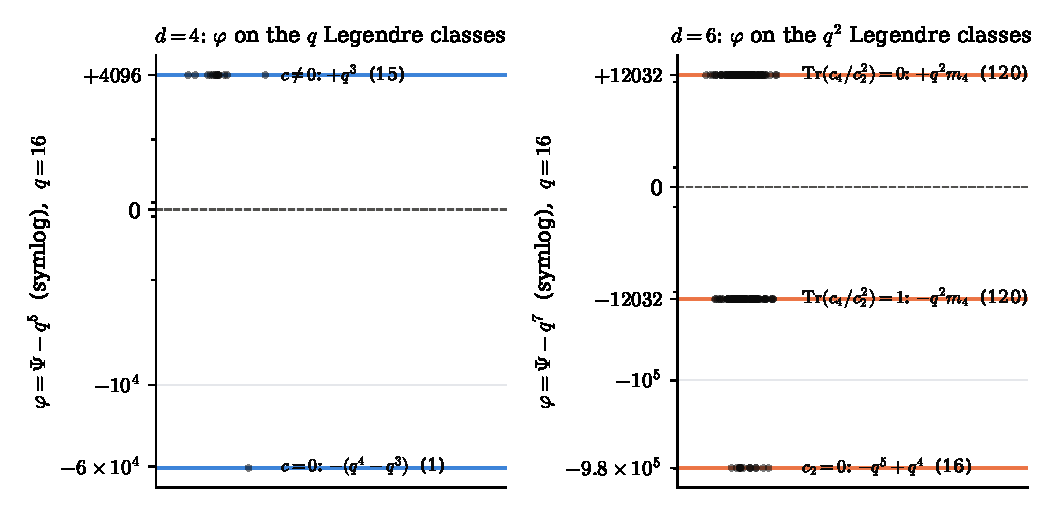
\includegraphics[width=\textwidth]{fig_profile.pdf}
\caption{The Legendre deviations $\varphi=\Psi-q^{d+1}$ for $q=16$. Left: $d=4$, the $q$ classes $(0,c,0)$ take the two values of Corollary~\ref{cor:d4}; the identity class carries $-(q^4-q^3)$. Right: $d=6$, the $q^2$ classes $(0,c_2,0,c_4,0)$ take exactly the three values of Theorem~\ref{thm:threevalue} ($m_4=47$). Each dot is one class (horizontal jitter only); the deviations are not continuous noise but are pinned to discrete levels by the translation symmetry of $U$.}\label{fig:profile}
\end{figure}

\begin{remark}
The same argument applies to every $d$: $U_d=\{p_j=0,\ j\text{ odd}\le\ell\}$ is stable under $\F_q$-translations and scalings, and the transformation law of $e_{2j}$ is governed by $\binom{2d-i}{2j-i}\bmod2$ (Lucas' theorem). For $d=4$ one recovers Corollary~\ref{cor:d4}(c).
\end{remark}

\section{The quadratic tower $\F_{q^{12}}\supset\F_{q^6}$}\label{sec:tower6}

\begin{lemma}\label{lem:towerC}
For $\alpha\in\F_{q^{12}}$ let $a=\alpha+\alpha^{q^6}$, $n=\alpha^{1+q^6}\in\F_{q^6}$, $\Tr=\Tr_{q^6/q}$, and $e_j(a)$ the elementary symmetric functions of the six conjugates of $a$. Then
\begin{align*}
e_1&=\Tr a,\qquad e_2=e_2(a)+\Tr n,\qquad e_3=e_3(a)+\Tr a\Tr n+\Tr(an),\\
e_4&=e_4(a)+e_2(a)\Tr n+e_1(a)\Tr(an)+\Tr(a^2n)+e_2(n),\\
e_5&=e_5(a)+e_3(a)\Tr n+e_2(a)\Tr(an)+e_1(a)\Tr(a^2n)+\Tr(a^3n)\\
&\qquad+e_1(a)e_2(n)+\Tr(an)\Tr n+\Tr(an^2),\\
p_3&=\Tr(a^3+an),\qquad p_5=\Tr(a^5+a^3n+an^2),
\end{align*}
and $e_2(\beta+\beta^q)=\Tr_{q^{12}/q}(\beta^{q+1})+(\Tr_{q^{12}/q}\beta)^2$ for all $\beta\in\F_{q^{12}}$. The multiplicity statement of Lemma~\ref{lem:towerA} holds verbatim with $\F_{q^4}$ replaced by $\F_{q^6}$; in particular $\F_{q^6}\subset U$, with $e_2|_{\F_{q^6}}=(\Tr\alpha)^2$ and $e_4|_{\F_{q^6}}=e_2(\alpha)^2$.
\end{lemma}
\begin{proof}
Expand $\prod_{i<6}(t^2+a_it+n_i)$ using $e_2(a\setminus j)=e_2(a)+a_je_1(a)+a_j^2$, $e_3(a\setminus j)=e_3(a)+a_je_2(a)+a_j^2e_1(a)+a_j^3$ and $e_1(a\setminus j,k)=e_1(a)+a_j+a_k$. The power sums follow from $s_k=as_{k-1}+ns_{k-2}$ for $s_k=\alpha^k+\alpha^{q^6k}$. All identities were also checked by exhaustive computation over $\F_{2^{12}}$.
\end{proof}

\begin{lemma}[Gauss sum of $e_2$]\label{lem:gauss}
On $\F_{q^6}$ the quadratic form $e_2$ has polar form $B(x,y)=\Tr x\Tr y+\Tr(xy)$, which is nondegenerate. For every $\beta\in\F_{q^6}$,
$\sum_{n\in\F_{q^6}}\chi(e_2(n)+\Tr(\beta n))=\chi(e_2(\beta))\,G$ with $G=\sum_n\chi(e_2(n))$.
\end{lemma}
\begin{proof}
$n_0=\beta+\Tr\beta$ satisfies $B(n_0,\cdot)=\Tr(\beta\,\cdot)$, and $e_2(\beta+c)=e_2(\beta)+c\Tr\beta+c^2$ for $c\in\F_q$ gives $e_2(n_0)=e_2(\beta)$.
\end{proof}

\begin{theorem}[tower reduction]\label{thm:towerred}
Let $a$ range over $\F_{q^6}\setminus\{0\}$ with $\Tr a=0$, $(\lambda,\mu)\in\F_q^2$, $\eps\in\{0,1\}$, and put
\[
\beta'=\lambda a+\sqrt\mu\sqrt a+\mu a^3+\eps a^{-2},\qquad \beta=e_2(a)+a^2+\beta',\qquad w=\chi(\lambda\Tr a^3+\mu\Tr a^5).
\]
Then
\begin{align*}
A_6&=q^6+q^4\sum_a\sum_{\beta'=0}(-1)^\eps w,\qquad
X=q^4\sum_a\chi(e_2(a))\sum_{\beta'=1}(-1)^\eps w,\\
Y&=G\Big[1+q^{-2}\sum_a\sum_{\lambda,\mu,\eps}(-1)^\eps\chi\bigl(e_4(a)+\lambda\Tr a^3+\mu\Tr a^5+e_2(\beta)\bigr)\Big].
\end{align*}
\end{theorem}
\begin{proof}
For $a\ne0$ with $\Tr a=0$, the conditions $p_3=p_5=0$ read $\Tr(an)=\Tr a^3$ and $\Tr(\sqrt a\,n)^2+\Tr(a^3n)=\Tr a^5$ (using $\Tr(an^2)=\Tr(\sqrt a\,n)^2$); expand their indicators and the irreducibility indicator $\frac12\sum_\eps(-1)^\eps\chi(\eps\Tr(a^{-2}n))$ by additive characters, using $\chi(\mu t^2)=\chi(\sqrt\mu\,t)$. The $n$-sums are $q^6[\gamma=0]$ for $A_6,X$ (no $e_2(n)$ term) and $\chi(e_2(\beta))G$ for $Y$ by Lemma~\ref{lem:gauss}. The contribution of $\alpha\in\F_{q^6}$ is $q^6$, $0$, $G$ respectively.
\end{proof}

\begin{remark}\label{rem:thin}
The equation $\beta'=0$ with $\eps=0$ and $\mu\ne0$ squares to $\mu^2a^5+\lambda^2a+\mu=0$, forcing $a\in\F_{q^2}\cup\F_{q^3}$ (a thin layer, as in Case II of Theorem~\ref{thm:d4formula}). For $\eps=1$, with $u=\mu a^5+\lambda a^3+1$ it becomes $u^2+u=\lambda a^3+1$: the points $(a,u)\in E_\lambda(\F_{q^6})$ of the supersingular elliptic curve $E_\lambda:y^2+y=\lambda x^3+1$ with $(u+\lambda a^3+1)/a^5\in\F_q$. The additional term $e_2(\beta)$ in $Y$ is quadratic in $(\lambda,\sqrt\mu)$ with cubic cross terms, which is why $Y$ does not collapse onto a thin layer.
\end{remark}

The reductions were verified numerically for $q=2,4,8$; they give $G=\sgn q^3$ for $k\le3$.

\section{Quadratic forms and supersingular Artin--Schreier curves}\label{sec:qf}

\subsection{$A_6$ and $X$ as sums of Frobenius traces}
\begin{theorem}\label{thm:supersing}
Write $\lambda=(\lambda_1,\lambda_3,\lambda_5)\in\F_q^3$ and $S(\lambda)=\sum_{x\in\F_{q^{12}}}\psi_0(\lambda_5x^5+\lambda_3x^3+\lambda_1x)$. Then
\begin{equation}\label{eq:A6S}
A_6-q^9=\frac1{q^3}\sum_{\lambda\ne0}S(\lambda),
\end{equation}
and $S(\lambda)=-\sum_j\omega_j(\lambda)^{12}$, where $\omega_j(\lambda)$ are the Frobenius eigenvalues over $\F_q$ of the Artin--Schreier curve $C_\lambda:y^2+y=\lambda_5x^5+\lambda_3x^3+\lambda_1x$ (genus $2$, $1$, $0$ according as $\lambda_5\ne0$; $\lambda_5=0\ne\lambda_3$; only $\lambda_1\ne0$). Moreover $\Tr_{q^{12}/2}(\lambda_5x^5+\lambda_3x^3)=Q_\lambda(x)$ is an $\F_2$-quadratic form with polar form $B_\lambda(x,y)=\Tr(y\,T_\lambda(x))$,
\[
T_\lambda(x)=\lambda_5x^4+(\lambda_5x)^{1/4}+\lambda_3x^2+(\lambda_3x)^{1/2},\qquad
R_\lambda=\ker T_\lambda=\{x:\lambda_5^4x^{16}+\lambda_3^4x^8+\lambda_3^2x^2+\lambda_5x=0\},
\]
so that $S(\lambda)\in\{0,\pm2^{(12k+r_\lambda)/2}\}$ with $r_\lambda=\dim_{\F_2}R_\lambda\le4$, $S(\lambda)=0$ iff $\Tr(\lambda_1x)\ne Q_\lambda(x)$ for some $x\in R_\lambda$, and the sign otherwise is the Arf invariant of $Q_\lambda$ on $\F_{q^{12}}/R_\lambda$ (shifted by $Q_\lambda(x_0)$, $B_\lambda(x_0,\cdot)=\Tr(\lambda_1\cdot)$). In particular all $C_\lambda$ are supersingular: $\omega_j(\lambda)=\sqrt q\,\zeta_j$ with roots of unity $\zeta_j$.
\end{theorem}
\begin{proof}
$A_6=\sum_{g\in\G^2}\Psi(g)=\frac{|\G^2|}{|\G|}\sum_{\eps^2=1}\psi_{12}(\eps)$ and $\psi_{12}(\eps_\lambda)=S(\lambda)$ by Proposition~\ref{prop:quadchar}; $S(0)=q^{12}$. The $L$-function interpretation is standard. $Q_\lambda(x)=\Tr(x(\lambda_5x^4+\lambda_3x^2))$ is of the form $\Tr(xL(x))$ with $L$ linearised, whence the quadratic-form statements; the kernel of $T_\lambda$ equals that of $T_\lambda^4$. Since the same structure persists over every $\F_{q^m}$, $\sum_{x\in\F_{q^m}}(-1)^{\Tr f_\lambda(x)}\in\{0,\pm2^{(mk+r)/2}\}$ for all $m$, which forces the normalised eigenvalues to be roots of unity \cite{GV}.
\end{proof}

Summing over $\lambda_1$ and using Hilbert~90 ($\alpha=\beta+\beta^q$, $\theta=\sigma+\sigma^{-1}$, $\Tr\alpha^3=\Tr(\beta^2\theta\beta)$, $\Tr\alpha^5=\Tr(\beta^4\theta\beta)$) one obtains the equivalent forms
\begin{equation}\label{eq:W}
A_6=q^9+\frac1{q^3}\sum_{(\lambda_3,\lambda_5)\ne0}W(\lambda_3,\lambda_5),\qquad
X=\frac1{q^3}\sum_{\lambda_3,\lambda_5}W'(\lambda_3,\lambda_5),
\end{equation}
with $W=\sum_\beta(-1)^{\Tr(\lambda_3\beta^2\theta\beta+\lambda_5\beta^4\theta\beta)}$ and $W'=\sum_\beta(-1)^{\Tr(\lambda_3\beta^2\theta\beta+\lambda_5\beta^4\theta\beta+\beta^{q+1}+\beta)}$ (the second uses Lemma~\ref{lem:towerC}). Their polar forms are $\Tr(\gamma M(\theta\beta))$ with $M(y)=\lambda_3y^2+\sqrt{\lambda_3y}+\lambda_5y^4+(\lambda_5y)^{1/4}$ ($+y$ for $W'$), so the radicals are $\theta^{-1}(\ker M\cap\im\theta)$, of dimension $2k+\dim(\ker M\cap\im\theta)$, where $\ker\theta=\F_{q^2}$ and $\im\theta=\ker\Tr_{q^{12}/q^2}$.

\subsection{The pure cubic part}
\begin{lemma}\label{lem:purecubic}
For all $k$ and all $\lambda_3\in\F_q^\times$: $W(\lambda_3,0)=0$ if $k$ is odd and $W(\lambda_3,0)=-2q^7$ if $k$ is even.
\end{lemma}
\begin{proof}
$\ker M=\{0\}\cup\{y:y^3=\lambda_3^{-1}\}$, and all three cube roots lie in $\F_{q^{12}}$. With $\zeta=y^{q-1}\in\mu_3$: $\zeta=1$ gives $y\in\F_q$; for $\zeta\ne1$, $k$ odd gives $y\in\F_{q^2}$ and $k$ even gives $y\in\F_{q^3}$. In all cases $\Tr_{q^{12}/q^2}y=0$, so $\ker M\subset\im\theta$ and $\dim R=2k+2$, $|W|\in\{0,2^{7k+1}\}$. Now $Q(\beta)=\Tr_{q^{12}/2}(\lambda_3\beta^2\theta\beta)$ vanishes on $\ker\theta$, and for $\theta\beta=y$ it is independent of the choice of $\beta$ (the ambiguity $c\in\F_{q^2}$ contributes $\Tr(\lambda_3c^2y)$ with $c^2y$ in a subfield of even index). If $y\in\F_{q^2}$, $\zeta\ne1$: on $\F_{q^4}$ one has $\theta\beta=\sigma(\Tr_{q^4/q^2}\beta)$, so pick $\beta_y\in\F_{q^4}$ with $\Tr_{q^4/q^2}\beta_y=y^q$; then
$Q(\beta_y)=\Tr_{q^4/2}(\lambda_3y\beta_y^2)=\Tr_{q^2/2}(\lambda_3y\,(\Tr_{q^4/q^2}\beta_y)^2)=\Tr_{q^2/2}(\lambda_3y^{2q+1})=\Tr_{q^2/2}(\zeta^2)=k\pmod2$, which is $1$ for $k$ odd: $Q|_R\ne0$ and $W=0$. If $y\in\F_q$ the same computation gives $\Tr_{q^2/2}(1)=0$; if $y\in\F_{q^3}$ ($k$ even) then $\Tr_{q^3/q}y=0$, $\theta$ is invertible on the trace-zero part of $\F_{q^3}$, $\beta_y\in\F_{q^3}$ and $Q(\beta_y)=0$. So for $k$ even $|W|=2q^7$. Finally $W=\sum_{\lambda_1\in\F_q}S(\lambda_1,\lambda_3,0)$ with $|S|=2q^6$ for each term ($r=2$), and $|W|=q\cdot2q^6$ forces all $q$ signs to agree with that of $S(0,\lambda_3,0)=-2q^6$ (Hasse--Davenport, $m=6k$).
\end{proof}

\begin{remark}
For $k$ odd the analogue of Lemma~\ref{lem:lambda1} fails over $\F_{q^{12}}$: the cube roots lie in $\F_{q^2}$ and $[\F_{q^6}:\F_{q^2}]=3$ is odd, so $\F_q\not\subset T(\F_{q^6})$. The vanishing of $W(\lambda_3,0)$ is exactly this failure.
\end{remark}

\subsection{Exact evaluation and the conjecture}
Every $W,W'$ is the exponential sum of an $\F_2$-quadratic form (plus a linear form) on $\F_2^{12k}$, hence computable exactly by linear algebra: radical, test of $Q+L$ on it, a symplectic basis of a complement and its Arf invariant. We implemented this (\texttt{legendre\_d6\_qf.py}) with $\F_{q^{12}}=\F_q[z]/(m)$ and the maps $\beta\mapsto\beta^2,\beta^{1/2},\sigma,\theta$ as $12k\times12k$ matrices over $\F_2$.

\begin{conjecture}\label{conj:A6X}
For all $q=2^k$: $A_6=q^9+\sgn(q-1)q^5$ and $X=\sgn\,q^6+q^5$, i.e.
\[
\sum_{\lambda_5\ne0}W(0,\lambda_5)+\sum_{\lambda_3\lambda_5\ne0}W(\lambda_3,\lambda_5)=(q-1)q^7(\sgn q+2),\qquad \sum_{\lambda_3,\lambda_5}W'(\lambda_3,\lambda_5)=q^3(\sgn q^6+q^5).
\]
\end{conjecture}

\begin{table}[ht]
\centering
\caption{Exact values of $A_6$ and $X$ by the quadratic-form algorithm ($N=12k$ bits). For $k\le5$ the values coincide with the Hayes-group FFT of \cite{Chen}; $k=6,7$ are beyond its reach at $d=6$. In all cases $A_6=q^9+(-1)^{k+1}(q-1)q^5$ and $X=(-1)^{k+1}q^6+q^5$.}\label{tab:A6X}
\begin{tabular}{@{}rrrrrr@{}}
\toprule
$k$ & $q$ & $N$ & $A_6$ & $X$ & time \\
\midrule
1 & 2 & 12 & $544$ & $96$ & $<1$ s\\
2 & 4 & 24 & $259\,072$ & $-3\,072$ & $<1$ s\\
3 & 8 & 36 & $134\,447\,104$ & $294\,912$ & $<1$ s\\
4 & 16 & 48 & $68\,703\,748\,096$ & $-15\,728\,640$ & $2$ s\\
5 & 32 & 60 & $35\,185\,412\,276\,224$ & $1\,107\,296\,256$ & $9$ s\\
6 & 64 & 72 & $18\,014\,330\,863\,747\,072$ & $-67\,645\,734\,912$ & $48$ s\\
7 & 128 & 84 & $9\,223\,376\,400\,541\,548\,544$ & $4\,432\,406\,249\,472$ & $225$ s\\
\bottomrule
\end{tabular}
\end{table}

\begin{table}[ht]
\centering
\caption{Distribution of $W(\lambda_3,\lambda_5)/q^7$ over the $q^2-1$ nontrivial pairs (radical dimension in parentheses); ``pure cubic'' $\lambda_5=0$, ``pure quintic'' $\lambda_3=0$, ``mixed'' $\lambda_3\lambda_5\ne0$.}\label{tab:W}
\begin{tabular}{@{}rlll@{}}
\toprule
$k$ & pure cubic ($q-1$) & pure quintic ($q-1$) & mixed ($(q-1)^2$)\\
\midrule
1 & $0$ (4) & $2$ (4) & $0$ (6) $\times1$\\
3 & $0$ (8) & $2$ (8) & $2$ (8) $\times21$; $0$ (10) $\times28$\\
5 & $0$ (12) & $2$ (12) & $2$ (12) $\times465$; $0$ (14) $\times496$\\
7 & $0$ (16) & $2$ (16) & $2$ (16) $\times8001$; $0$ (18) $\times8128$\\
\midrule
2 & $-2$ (6) & $0$ (8) & $-4$ (8) $\times3$; $1$ (4) $\times6$\\
4 & $-2$ (10) & $-4$ (12) $\times3$; $1$ (8) $\times12$ & $-4$ (12) $\times75$; $1$ (8) $\times90$; $0$ (12) $\times60$\\
6 & $-2$ (14) & $0$ (16) & $-4$ (16) $\times1386$; $1$ (12) $\times1638$; $0$ (16) $\times945$\\
\bottomrule
\end{tabular}
\end{table}

\begin{proposition}[structure of the data]\label{prop:pattern}
For $k\le7$ the following hold.
\begin{enumerate}[label=\textup{(\alph*)},leftmargin=2em]
\item $k$ odd: $W(0,\lambda_5)=2q^7$ for all $\lambda_5\ne0$; the mixed $W$ depends only on $j=\lambda_3^5/\lambda_5^3\in\F_q^\times$ and equals $2q^7$ for exactly $(q-2)/2$ values of $j$ and $0$ otherwise. Hence $\sum W=(q-1)\,2q^7+\frac{(q-1)(q-2)}2\,2q^7=(q-1)q^8$.
\item $k$ even: $W(0,\lambda_5)=0$ if $k\equiv2\pmod4$, while for $k\equiv0\pmod4$ (so $5\mid q-1$) it equals $-4q^7$ for the $(q-1)/5$ fifth powers and $+q^7$ otherwise; the mixed $W$ take values $-4q^7,\ q^7,\ 0$ with multiplicities $(q-1)(n_-,n_+,n_0)$, $(n_-,n_+,n_0)=(1,2,0),(5,6,4),(22,26,15)$ for $k=2,4,6$, satisfying $n_+-4n_-=2-q$.
\end{enumerate}
The set of $j$ in (a) is not of the form $\{\Tr_{q/2}(j^m)=c\}$ for any $m$ when $k=5,7$ (it is $\{\Tr j=0\}$ when $k=3$).
\end{proposition}

Conjecture~\ref{conj:A6X} is thus equivalent to a precise statement about which radicals $\theta^{-1}(\ker M\cap\im\theta)$ carry a vanishing $Q$ and about the Arf invariants, for the $15$-th degree linearised polynomials $\lambda_5^4y^{15}+\lambda_3^4y^7+\lambda_3^2y+\lambda_5$. The supersingular point counts of Theorem~\ref{thm:supersing} determine the possible absolute values; they do not by themselves decide which pairs $(\lambda_3,\lambda_5)$ vanish. We leave the pure quintic and mixed cases open.

\section{The scaling law at $d=6$ and the nature of $Y$}\label{sec:Y}

\subsection{Variance formula}
\begin{theorem}\label{thm:varH6}
Assume Conjecture~\ref{conj:A6X} (true for $q\le128$) and write $Y=q^3m_k$. Then $B=-2q^3[k\text{ odd}]$,
\[
\varphi_0=\begin{cases}q^5+q^4-2q^3,&k\text{ odd},\\-q^5+q^4,&k\text{ even},\end{cases}\qquad
\varphi_{A,B}=\begin{cases}-2q^3\pm q^2m_k,&k\text{ odd},\\ \pm q^2m_k,&k\text{ even},\end{cases}
\]
and
\[
\frac{\Var_{\G^2}(\Psi)}{q^7}=\begin{cases}\dfrac{(q-1)^2(q+2)^2}{q^2}+\dfrac{(q-1)(4q^2+m_k^2)}{q^4},&k\text{ odd},\\[2ex](q-1)^2+\dfrac{(q-1)m_k^2}{q^4},&k\text{ even}.\end{cases}
\]
In particular $\Var_{\G^2}(\Psi)/q^7=q^2(1+O(1/q))$, i.e.\ $C_6:=\lim_{q\to\infty}\Var_{\G^2}(\Psi)/q^9=1$, provided $m_k=o(q^{5/2})$.
\end{theorem}
\begin{proof}
Substitute into Corollary~\ref{cor:profile}.
\end{proof}

\begin{table}[ht]
\centering
\caption{$d=6$: exact variances (Hayes FFT, $q\le32$; $q=16$ also by CRT), the three Legendre deviations and $m_k=Y/q^3$. The last two columns show that $\Var_{\G^2}/q^7\asymp q^2$ and not $q^4$.}\label{tab:d6var}
\begin{tabular}{@{}rrrrrrrrr@{}}
\toprule
$q$ & $\Var_\G/q^7$ & $\Var_{\G^2}/q^7$ & ratio & $\varphi_0$ & $\varphi_A$ & $\varphi_B$ & $m_k$ & $\Var_{\G^2}/q^9$\\
\midrule
2 & 5.7578 & 15.5625 & 2.703 & $32$ & $36$ & $-68$ & $13$ & 3.891\\
4 & 3.7004 & 9.0117 & 2.435 & $-768$ & $-16$ & $16$ & $-1$ & 0.563\\
8 & 4.7483 & 79.0935 & 16.657 & $35\,840$ & $-3\,264$ & $1\,216$ & $-35$ & 1.236\\
16 & 4.3514 & 225.5056 & 51.824 & $-983\,040$ & $12\,032$ & $-12\,032$ & $47$ & 0.881\\
32 & 4.2086 & 1100.8844 & 261.581 & $34\,537\,472$ & $685\,056$ & $-816\,128$ & $733$ & 1.075\\
\bottomrule
\end{tabular}
\end{table}

\begin{figure}[ht]
\centering
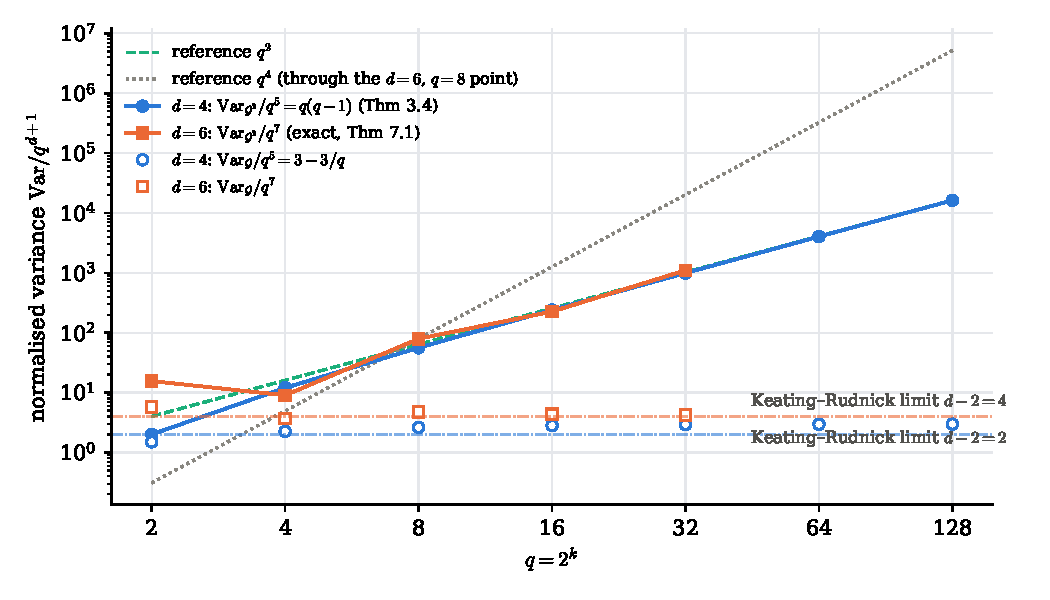
\includegraphics[width=0.95\textwidth]{fig_scaling.pdf}
\caption{Normalised variances against $q$ (log--log). Filled markers: $\Var_{\G^2}(\Psi)/q^{d+1}$, exact values ($d=4$: $q(q-1)$ for $q\le128$, Theorem~\ref{thm:varH4}; $d=6$: Table~\ref{tab:d6var}). Open markers: the full-group variances $\Var_\G/q^{d+1}$, which approach $3$ ($d=4$, Theorem~\ref{thm:varG4}) and the Keating--Rudnick value $4$ ($d=6$). The dashed line is $q^2$; the dotted line is a $q^4$ law normalised through the $d=6$, $q=8$ point, which the data exclude. Whether $\lim\Var_{\G^2}/q^{9}=1$ at $d=6$ depends on $m_k=o(q^{5/2})$ (Theorem~\ref{thm:varH6}).}\label{fig:scaling}
\end{figure}

\begin{remark}
At $d=4$ the Legendre anomaly is a single class with relative deficit $1/q$; at $d=6$ it is the $q$ classes with $c_2=0$ (the intervals around $f^2$ with $f_5=0$), each with relative deviation $\pm q^{-2}$ and sign $\sgn$. Both mechanisms give $\Var_{\G^2}/q^{d+1}\asymp q^2$. The full-group variance $\Var_\G/q^7$ tends to the Keating--Rudnick value $4$ ($4.35,4.21$ at $q=16,32$), unlike $d=4$ where it tends to $3\ne2$. The value $q^{2(d/2-1)}=q^4$ suggested in \cite{Chen} is excluded.
\end{remark}

\subsection{The geometry behind $Y$: a fixed nine-dimensional variety and a twisted Frobenius}\label{subsec:Ygeom}

We now give $Y$ an unambiguous algebro-geometric meaning. The point is that $Y_k$ is a Frobenius trace on a \emph{fixed} variety over $\F_2$, but for a \emph{twisted} Frobenius; in particular $(Y_k)_k$ is not the sequence of $\F_{2^k}$-point counts of any single variety.

\begin{definition}\label{def:X}
Let $z=(z_0,\dots,z_{11})$ be coordinates on $\A^{12}_{\F_2}$ and $e_m(z)$ the elementary symmetric polynomials. Put
\[
I=\langle e_1,e_3,e_5\rangle\subset\F_2[z],\qquad X=V(I)\subset\A^{12}_{\F_2},\qquad f=e_4|_X,\qquad \mathcal L=f^*\mathcal L_{\psi_0},
\]
where $\mathcal L_{\psi_0}$ is the Artin--Schreier sheaf on $\A^1_{\F_2}$ attached to $\psi_0(x)=(-1)^x$, so that the trace function of $\mathcal L\otimes\F_q$ is $\psi_q\circ e_4$. Let $\sigma\in\mathrm{Aut}(\A^{12})$ be the cyclic shift $\sigma(z)_j=z_{j-1}$ (indices mod $12$); it is defined over $\F_2$, preserves $I$ and $e_4$, and commutes with the absolute Frobenius $F:z\mapsto(z_j^2)$. The $\sigma$-twisted $\F_q$-form $X^{(\sigma)}$ of $X$ is the $\F_q$-structure whose geometric Frobenius is $\sigma\circ F^k$ (the class of a $12$-cycle in $H^1(\F_q,S_{12})$; it is the twist defining $\mathrm{Res}_{\F_{q^{12}}/\F_q}\A^1\cong\A^{12}_{\F_q}$).
\end{definition}

\begin{proposition}\label{prop:trace}
\begin{enumerate}[label=\textup{(\alph*)},leftmargin=2em]
\item $I=\langle p_1,p_3,p_5\rangle$ with $p_m=\sum_jz_j^m$ (Newton's identities in characteristic $2$: $p_3=e_1^3+e_1e_2+e_3$, $p_5\equiv e_5+e_2e_3\pmod{e_1}$).
\item $\alpha\mapsto(\alpha,\alpha^q,\dots,\alpha^{q^{11}})$ is a bijection $U\to X^{(\sigma)}(\F_q)=\{z\in X(\bar\F_2):\sigma F^k(z)=z\}$ carrying $e_4(\alpha)$ to $e_4(z)$; hence $Y=\sum_{z\in X^{(\sigma)}(\F_q)}\psi_q(e_4(z))$.
\item Let $\pi:\A^{12}\to\A^{12}/S_{12}=\mathrm{Spec}\,\F_2[e_1,\dots,e_{12}]$ and $\Lambda=V(e_1,e_3,e_5)\cong\A^9$ with coordinates $(e_2,e_4,e_6,e_7,\dots,e_{12})$. Then $X=\pi^{-1}(\Lambda)$, $\pi|_X:X\to\Lambda$ is finite flat of degree $12!$ and generically \'etale, $\Lambda(\F_q)$ is the set of monic $F\in\F_q[t]$ of degree $12$ with $a_{11}=a_9=a_7=0$, and $\#(\pi^{-1}(F)\cap X^{(\sigma)}(\F_q))=\Lambda(F)$. Thus $Y=\sum_{F\in\Lambda(\F_q)}\Lambda(F)\psi_q(a_8(F))$, which is the Hayes-group form of Section~\ref{sec:d6}; the projection $\Lambda\to\A^2$, $(e_2,e_4)$, has fibres of dimension $7$.
\end{enumerate}
\end{proposition}
\begin{proof}
(a) is immediate from Newton's identities. (b): $\sigma F^k(z)_j=z_{j-1}^q$, so the fixed points are the tuples $z_j=z_0^{q^j}$ with $z_0^{q^{12}}=z_0$, and $e_1=e_3=e_5=0$ is $p_1=p_3=p_5=0$ by (a). (c): $\F_2[z]$ is free of rank $12!$ over $\F_2[e]$; the generic $F$ is separable since $F'=e_7t^4+e_9t^2+e_{11}\ne0$; the $\sigma F^k$-fixed points of $\pi^{-1}(F)$ are the orderings $z_j=z_0^{q^j}$ of the roots of $F$, i.e.\ the $\alpha\in\F_{q^{12}}$ with $\charpoly(\alpha)=F$, of which there are $\Lambda(F)$ (cf.\ \eqref{eq:rootcount}).
\end{proof}

\begin{proposition}[geometry of $X$]\label{prop:Xgeom}
\begin{enumerate}[label=\textup{(\alph*)},leftmargin=2em]
\item $X$ is a complete intersection of codimension $3$ in $\A^{12}$ cut out by the regular sequence $(e_1,e_3,e_5)$ of degrees $1,3,5$; it is an affine cone of pure Krull dimension $9$ and is Cohen--Macaulay. (``Nine-dimensional'' refers to $\dim X$; the fibres of $X\to\Lambda$ have dimension $0$ and those of $X\to\A^2$ dimension $7$.)
\item $\mathrm{Sing}(X)=X\cap\{z:\#\{z_0,\dots,z_{11}\}\le2\}$ is the union of the $1023$ planes $P_A=\{z_j=u\ (j\in A),\ z_j=v\ (j\notin A)\}$, $A\subset\{0,\dots,11\}$ of even cardinality $0<|A|<12$ ($A$ and its complement give the same plane), all containing the diagonal line; $\dim\mathrm{Sing}(X)=2$, of codimension $7$.
\item $X$ is geometrically integral and normal. Consequently the geometric monodromy group of the family $\{F:e_1=e_3=e_5=0\}$, i.e.\ the Galois group of $t^{12}+e_2t^{10}+\dots+e_{11}t+e_{12}$ over $\bar\F_2(e_2,e_4,e_6,\dots,e_{12})$, is the full $S_{12}$.
\end{enumerate}
\end{proposition}
\begin{proof}
(a) By Proposition~\ref{prop:trace}(c), $\F_2[z]/I$ is a free module over $\F_2[e]/(e_1,e_3,e_5)\cong\F_2[e_2,e_4,e_6,\dots,e_{12}]$, so $(e_1,e_3,e_5)$ is a regular sequence and $X$ is finite over $\A^9$. (b) By the Jacobian criterion for complete intersections, $X$ is smooth at $z$ iff $de_1,de_3,de_5$ are independent there. On $X$, $\partial_je_1=1$, $\partial_je_3=e_2(z\setminus z_j)=e_2+z_j^2$ and $\partial_je_5=e_4(z\setminus z_j)=e_4+e_2z_j^2+z_j^4$, so the row space is that of the Vandermonde rows $(1)_j,(z_j^2)_j,(z_j^4)_j$, of rank $3$ iff at least three of the $z_j$ are distinct. Conversely, if $z$ takes only the values $u,v$ with multiplicities $s,r$, $s+r=12$, then $e_m(z)=\sum_i\binom{s}{m-i}\binom ri u^{m-i}v^i$; for $r$ even every term with $m$ odd contains a factor $\binom{\mathrm{even}}{\mathrm{odd}}$, which is even by Lucas' theorem, so $e_1=e_3=e_5=0$ and $P_A\subset X$; for $r$ odd, $e_1=u+v$ forces $u=v$. (c) $X$ is generically reduced (generic fibre of $\pi$ \'etale) and Cohen--Macaulay, hence reduced; Cohen--Macaulay gives Serre's $S_2$ and (b) gives $R_1$, so $X$ is normal; a cone is connected, and a connected normal variety is irreducible. The same holds over $\bar\F_2$. The irreducible components of $X_{\bar\F_2}$ correspond to the cosets $S_{12}/G$ of the geometric monodromy group $G$ (the generic fibre of $\pi$ is the splitting algebra), so $G=S_{12}$.
\end{proof}

\begin{proposition}[the Artin--Schreier sheaf]\label{prop:ASsheaf}
The cover $Z=\{(z,y)\in X\times\A^1:y^2+y=e_4(z)\}\to X$ is \'etale of degree $2$ and $Z$ is smooth over $X_{\rm sm}$. The function $f=e_4$ has no poles on $X$; on the projective closure $\overline X\subset\mathbb P^{12}$ its polar divisor is $4X_\infty$ with $X_\infty\cong\mathbb P(X)\subset\mathbb P^{11}$ the base of the cone. Since the pole order $4$ is divisible by $p=2$, the Swan conductor of $\mathcal L$ along $X_\infty$ is $<4$. The sheaf $\mathcal L$ is geometrically nontrivial on $X$ (on the diagonal line $e_4=\binom{12}4u^4=u^4$, and $u^4\notin\{g^2+g+c\}$), so $Z$ is geometrically connected and
\[
H^{18}_c(X_{\bar\F_2},\mathcal L)=H^0(X_{\bar\F_2},\mathcal L^\vee)^\vee(-9)=0 .
\]
\end{proposition}

\begin{theorem}[twisted trace formula]\label{thm:twisted}
For every $k\ge1$, with $F$ the geometric Frobenius of $\F_2$ acting on $\ell$-adic cohomology ($\ell\ne2$) and $\sigma$ acting through its lift to $\mathcal L$,
\[
Y_k=\sum_{j=0}^{18}(-1)^j\Tr\bigl(\sigma\circ F^k\;\big|\;H^j_c(X_{\bar\F_2},\mathcal L)\bigr).
\]
Consequently $\sum_{k\ge1}Y_kT^k=T\frac{d}{dT}\log L_\sigma(T)$ with $L_\sigma(T)=\prod_j\det(1-\sigma FT\mid H^j_c)^{(-1)^{j+1}}\in\mathbb Q(T)$; $(Y_k)_k$ is a linear recurrence sequence, and $m_k=Y_k/8^k=\sum_i\pm\zeta_i\eta_i^k$ with $\zeta_i^{12}=1$ and $\eta_i=\lambda_i/8$, $\lambda_i$ the eigenvalues of $F$. By Deligne \cite{Deligne} the $\lambda_i$ on $H^j_c$ are algebraic integers of weight $\le j$; the normalisation $8^k=q^3$ is the Tate twist by $3$, so $H^j_c(3)$ has weights $\le j-6$. If the cohomology were concentrated in degree $9=\dim X$ and pure, then $m_k=\pm\sum_{i=1}^{b_9}\zeta_i\eta_i^k$ with $|\eta_i|=2^{3/2}$ and $|m_k|\le b_9\,q^{3/2}$.
\end{theorem}
\begin{proof}
By Proposition~\ref{prop:trace}(b), $Y_k$ is the sum of the trace function of $\mathcal L$ over the $\F_q$-points of the twisted form $X^{(\sigma)}$, whose geometric Frobenius acts on $H^\bullet_c(X_{\bar\F_2},\mathcal L)$ as $\sigma F^k$ ($\sigma$ has finite order and commutes with $F$); apply the Grothendieck--Lefschetz formula (SGA~4$\frac12$, Rapport; for $F\circ\sigma$ with $\sigma$ of finite order see also Deligne--Lusztig \cite[proof of Thm.~3.2]{DL}). Since $\sigma$ and $F$ commute they are simultaneously triangularisable, which gives the stated shape; $L_\sigma$ has coefficients in $\mathbb Q(\zeta_{12})$ a priori and in $\mathbb Q$ because all $Y_k\in\mathbb Z$. The weight statements are Weil~II.
\end{proof}

By contrast with $A_6$ and $X$, the function $(-1)^{\Tr e_4}$ on $\G^2$ is not a character: in Witt coordinates $\G^2\cong W_2(\F_q)$, $(x_1,x_2)+(x_1',x_2')=(x_1+x_1',x_2+x_2'+x_1x_1')$, and the carry destroys multiplicativity (the characters of order $4$ are $i^{\Tr x_1}(-1)^{\Tr x_2+\cdots}$). Therefore $Y$ does not decompose into Frobenius traces of individual $L$-functions of curves and no supersingularity argument applies; it is the global twisted trace on the nine-dimensional $X$.

\begin{proposition}\label{prop:Ydata}
The values $m_k=13,-1,-35,47,733$ ($k=1,\dots,5$) satisfy $|m_k|/q^{3/2}=4.60,\,0.13,\,1.55,\,0.73,\,4.05$. Hence, in the pure, degree-$9$ situation of Theorem~\ref{thm:twisted}, $b_9\ge5$. The elementary symmetric functions of the $\zeta_i\eta_i$ computed from $m_1,\dots,m_5$ by Newton's identities are $13,85,361,1069,2281$; if $b_9=5$ then $|e_5|=\prod|\eta_i|=2^{15/2}\ne2281$, a contradiction (the argument uses only absolute values, so the twists $\zeta_i$ do not affect it). Thus either $b_9\ge6$, or $H^\bullet_c$ has contributions outside the pure weight-$9$ part.
\end{proposition}

\begin{sloppypar}
Proposition~\ref{prop:trace}(b) was checked directly: enumerating $X^{(\sigma)}(\F_2)$ inside $\F_{2^{12}}$ gives $|U|=544$, $Y_1=104$, and the pushforward formula of (c) gives $(|U|,Y)=(544,104)$ and $(259072,-64)$ for $q=2,4$ (script \texttt{verify\_Y\_direct.py}; a SageMath version is \texttt{verify\_Y\_sage.sage}).
\end{sloppypar}

\begin{remark}[what is and is not established]
Theorem~\ref{thm:twisted} and Propositions~\ref{prop:trace}--\ref{prop:ASsheaf} are unconditional. We have \emph{not} shown that $H^j_c(X_{\bar\F_2},\mathcal L)$ vanishes for $9<j<18$ (Proposition~\ref{prop:ASsheaf} gives only $j=18$), nor computed $b_9$: Katz's theorem on the concentration of $\sum\psi(f)$ in middle degree requires $p\nmid\deg f$ and a smooth ambient variety, whereas here $\deg e_4=4$ and $X$ is singular along the $1023$ planes of Proposition~\ref{prop:Xgeom}(b); a proof would need the Swan conductor of $\mathcal L$ along $X_\infty$ and local computations at $\mathrm{Sing}(X)$. Hence $m_k=O(q^{3/2})$, and with it $C_6=1$, is supported by the data but not proved. Two further cautions. First, the variety $V=\{p_1=p_3=p_5=0\}\subset\A^{12}_{\F_q}$ obtained by choosing an $\F_q$-basis of $\F_{q^{12}}$ is exactly $X^{(\sigma)}$, a nontrivial twist of $X\otimes\F_q$; so $(Y_k)_k$ is not a point-count sequence of a fixed variety, and the genuine ``closed form'' of $Y$ is the twisted $L$-function $L_\sigma(T)$, which Theorem~\ref{thm:twisted} shows is a rational function determined by finitely many $Y_k$ (Berlekamp--Massey on $Y_1,Y_2,\dots$ would identify it; $k\le5$ is not enough and $k=6$ means $\F_{2^{72}}$). Second, the untwisted counts $\#X(\F_q)$ for $q=2,4,8$ ($2048$, $2\,099\,200$, $1\,081\,081\,856$) far exceed $q^9$; this is not a sign of several components but of $q<12$, where no polynomial over $\F_q$ has twelve distinct roots. The tower reduction of Theorem~\ref{thm:towerred} exhibits $Y/G-1$ as a sum over $a\in\F_{q^6}$ of cubic Artin--Schreier sums over $\F_q$, i.e.\ as the trace of a relative $H^1$ of an elliptic Artin--Schreier family over a five-dimensional base; this is the natural starting point for computing $b_9$.
\end{remark}

\section{Summary of the numerical evidence}\label{sec:numerics}

\begin{table}[ht]
\centering
\caption{Status of the main identities. ``exact'' means verified by exact integer computation; the method is indicated.}\label{tab:status}
\small
\begin{tabular}{@{}p{0.42\textwidth}p{0.24\textwidth}p{0.3\textwidth}@{}}
\toprule
Statement & Status & Range checked\\
\midrule
$d=4$: Theorem~\ref{thm:d4formula} (all classes) & proved & formula $=$ FFT class by class, $q\le128$\\
$d=4$: $\Var_{\G^2}/q^5=q(q-1)$, $\Var_\G/q^5=3-3/q$ & proved & Lemma~\ref{lem:sigma} also checked to $q=2^{22}$\\
$d=4$: $\rho$ structure (Theorem~\ref{thm:rho4}) & proved & matches \cite[Table 4]{Chen}\\
$d=6$: three-value profile (Theorem~\ref{thm:threevalue}) & proved & all $q^2$ classes, $q\le32$\\
$d=6$: tower identities and reductions & proved & $\F_{2^{12}}$ exhaustive; $q=2,4,8$\\
$d=6$: $A_6,X$ closed forms (Conjecture~\ref{conj:A6X}) & open; pure cubic part proved & exact, $q\le128$ (Table~\ref{tab:A6X})\\
$d=6$: $\Var_{\G^2}/q^7$ formula (Theorem~\ref{thm:varH6}) & proved given Conj.~\ref{conj:A6X} & $q\le32$\\
$C_6=1$ & conditional on $m_k=o(q^{5/2})$ & $q\le32$\\
\bottomrule
\end{tabular}
\end{table}

\begin{thebibliography}{99}
\bibitem{Carlitz} L.~Carlitz, \emph{Explicit evaluation of certain exponential sums}, Math.\ Scand.\ \textbf{44} (1979), 5--16.
\bibitem{Chen} R.~Chen, \emph{Primes in Legendre intervals over $\F_q[t]$: an exact explicit-formula algorithm, verification for $d\le10$, and an anomaly in characteristic~2}, preprint (2026), DOI 10.5281/zenodo.23219609.
\bibitem{Coulter} R.~S.~Coulter, \emph{On the evaluation of a class of Weil sums in characteristic $2$}, New Zealand J.\ Math.\ \textbf{28} (1999), 171--184.
\bibitem{Deligne} P.~Deligne, \emph{La conjecture de Weil. II}, Publ.\ Math.\ IHES \textbf{52} (1980), 137--252.
\bibitem{DL} P.~Deligne and G.~Lusztig, \emph{Representations of reductive groups over finite fields}, Ann.\ of Math.\ (2) \textbf{103} (1976), 103--161.
\bibitem{GV} G.~van der Geer and M.~van der Vlugt, \emph{Reed--Muller codes and supersingular curves. I}, Compositio Math.\ \textbf{84} (1992), 333--367.
\bibitem{HD} H.~Hasse and H.~Davenport, \emph{Die Nullstellen der Kongruenzzetafunktionen in gewissen zyklischen F\"allen}, J.\ reine angew.\ Math.\ \textbf{172} (1935), 151--182.
\bibitem{Katz} N.~M.~Katz, \emph{Witt vectors and a question of Keating and Rudnick}, Int.\ Math.\ Res.\ Not.\ IMRN (2013), 3613--3638.
\bibitem{KR} J.~P.~Keating and Z.~Rudnick, \emph{The variance of the number of prime polynomials in short intervals and in residue classes}, Int.\ Math.\ Res.\ Not.\ IMRN (2014), 259--288.
\bibitem{LMW} J.~Lahtonen, G.~McGuire and H.~N.~Ward, \emph{Gold and Kasami--Welch functions, quadratic forms, and bent functions}, Adv.\ Math.\ Commun.\ \textbf{1} (2007), 243--250.
\end{thebibliography}

\end{document}
